\documentclass[a4paper,oneside,article, titlepage]{article}
\usepackage[T1]{fontenc}
\usepackage{textcomp}
\usepackage[utf8]{inputenc}
\usepackage[danish]{babel}
\usepackage[garamond]{mathdesign}
\usepackage{graphicx}

\DeclareTextFontCommand{\textfleur}
{\fontencoding{T1}\fontfamily{FleurCornerCaps}\selectfont}


\renewcommand{\ttdefault}{pcr} % bedre typewriter font
\renewcommand{\rmdefault}{ugm} % garamond


\usepackage{lettrine}

%\overfullrule=5pt

%\setsecnumdepth{part}

\title{Baselinedesign til hjemmesideanalyse  \\
       \small{Førsteårsprojekt}}

\author
{
  Gruppe 1:\\
  Troels Henriksen (athas@sigkill.dk)\\
  Jesper Reenberg (reenberg@kampsax.dtu.dk)\\
  Martin Dybdal (dybber@dybber.dk)\\ \\
  Vejledere: Dina og Kasper
}


\setcounter{tocdepth}{3}
\setcounter{secnumdepth}{2}

\pagestyle{plain}

\date{\today}

\begin{document}
\maketitle
\tableofcontents
\newpage

\section{Overordnet designfilosofi}

Vores program er ikke interaktivt, men kører derimod som et {\em
  batch--job} med en fra starten af veldefineret afslutning (når alle
sider er blevet analyseret), i modsætning til interaktive programmer,
som kører indtil brugeren vælger at afslutte dem. Da programmet
ydermere er baseret på at foretage gradvist mere raffinerede
bearbejdninger af det indkommende data har vi valgt at lave et
overordnet {\em dataflow}--design som beskriver hvordan data bliver
ført rundt i programmet. Programmeringssproget Standard ML er velegnet
til en sådan opgave --- manglen på objektorienterede faciliteter vil
ikke blive mærket, og programmets relativt korte og simple kørselstid
betyder at manglen på mutérbar tilstand ikke vil være et problem.

Her følger vores Dataflow diagram.
\subsection{Dataflow diagram}
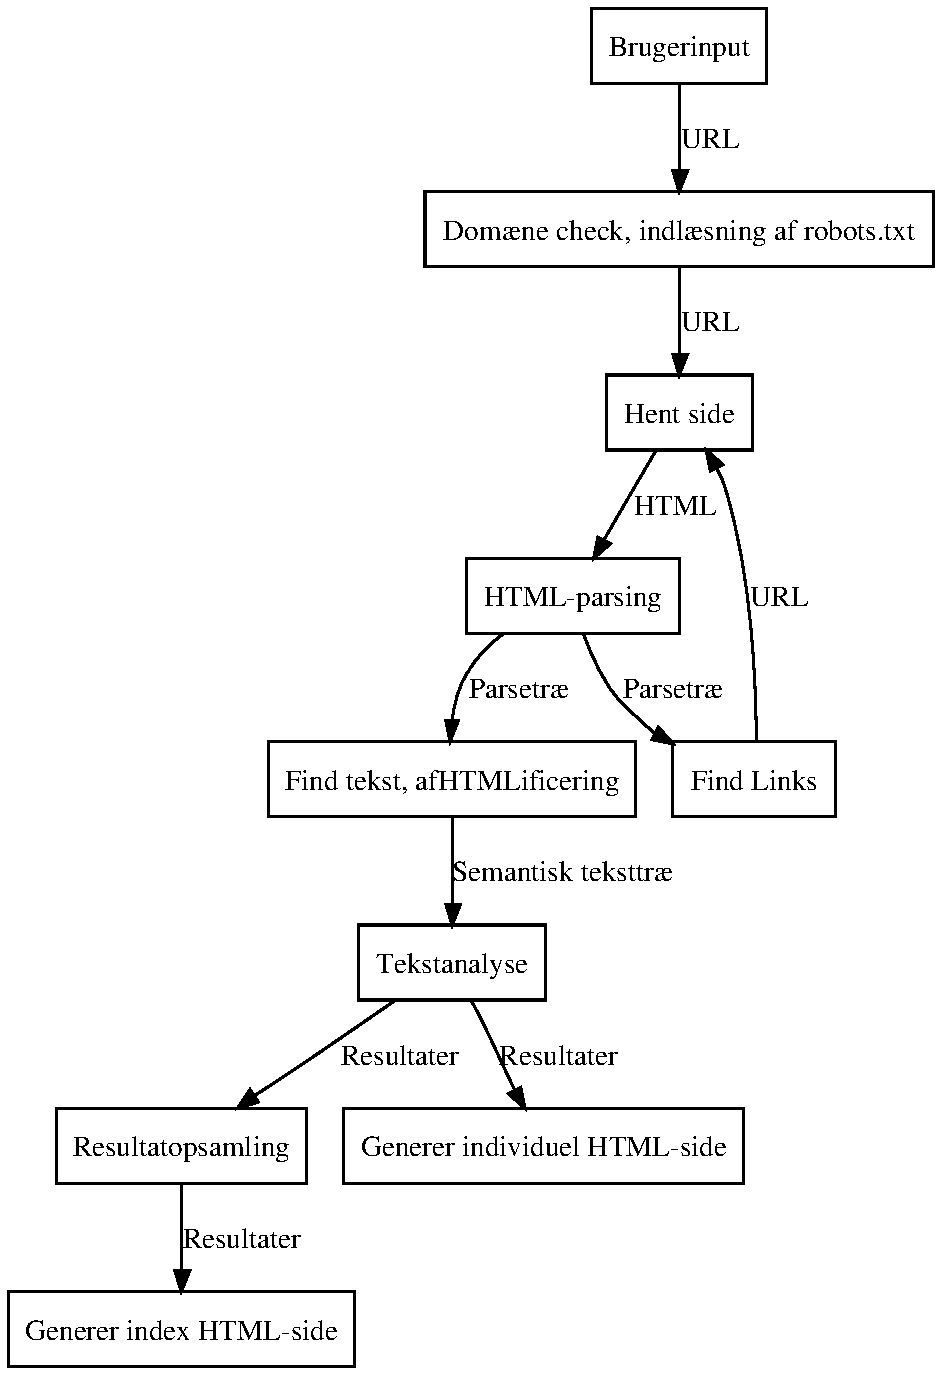
\includegraphics{designill.pdf}


\section{Moduler}
Vi vil nu beskrive de moduler vi har inddelt programmet i.

\subsection{Brugerinput}
Dette modul skal sætte en analyse i gang ud fra de parametre brugeren
angiver. Det skal også parse kommandolinjeparametrene og videregive
brugerindstillingerne til de andre moduler i programmet. Hvis
kommandolinjen er i et ugyldigt format, eller der er angivet ukendte
indstillinger, er det også dette moduls ansvar at informere brugeren
om fejlen og afslutte programmet.

\subsection{Domæne check, indlæsning af robots.txt}
Dette modul skal tjekke om det domæne brugeren har angivet kan tilgås
og give en fejlmeddelelse hvis det ikke er tilfældet. Hvis brugeren
har angivet det skal det undersøges om der er en \textit{robots.txt}
fil på serveren og hvis det er tilfældet så skal den
parses. Informationerne i \textit{robots.txt} skal gøres tilgængeligt
for \textit{Hent side}--modulet, så det kan se hvilke dele af websitet
det må crawle.

\subsection{Hent Side}
Hent side modulet skal kunne hente en side fra en webserver via
HTTP-protokollen. Da vores behov er små og vi ikke har for meget tid
vil vi bruge et eksternt produceret
Http-modul\footnote{http://www.diku.dk/undervisning/2000e/dat0/filer200001/K1/brevkasse.html},
modificeret til vores behov. Det er også dette moduls job at tjekke om
robots.txt tillader at vi må crawle siden, da dette skal tjekkes hver
gang der skal hentes en side.

\subsection{HTML-Parsing}
For at kunne udtrække tekst fra en HTML-side er det nødvendigt først
at parse den. Da vi ikke har været i stand til at finde en HTML-parser
skrevet i SML har vi valgt at implementere denne selv. Resultatet af
HTML-parsingen er et ordinært parsetræ som så i senere moduler bruges
til både at danne et mere højniveau-træ over teksten, og til at finde
links til andre sider som skal hentes.

Parseren er, for at lette implementationen, opdelt i to primære dele -
en lexer, der opdeler den inkommende sekvens af tegn i en liste af
leksikalske enheder uden nærmere struktur, og en egentlig parser, som
omdanner listen af de leksikale enheder til et struktureret
parsetræ. Lexeren er specificeret med en SML-signatur, men det er ikke
hensigten at denne bruges af andet end parser-modulet, og resten af
programmet vil ikke være påvirket af parsertrinnets toparts-opdeling.

De leksikale enheder produceret af lexeren vil være af tre forskellige
typer - begyndelsestags, afslutningstags og tekstelementer. De to
tag-typer vil indeholde information om navnet på det relevante tag,
samt en liste indeholdende attribut/værdi-tupler. Tekstelementer vil
indeholde information om den sekvens af tegn de repræsenterer.

Det af parseren producerede parsetræ består af knuder, repræsenterende
tags, og blade, repræsenterende tekst. En knude kan have nul eller
flere undergrene der angiver de HTML-elementer der findes mellem
start- og slut-tagget (nul undergrene kunne f.eks. være et
``\texttt{<br />}''-element), hvor hver undergren igen kan være enten
en knude eller et blad. For eksempel vil HTML-strengen
``\texttt{<strong>}\texttt{<em>}Vigtigt!\texttt{</em>} Parseren skal
fungere\texttt{</strong>}'' bestå af en knude med to undergrene -
endnu en knude og et blad indeholdende tekst. Undergrenene skal være
ordnede i samme rækkefølge som deres optræden i det oprindelige
HTML-dokument. En knude indeholder information om hvilket tag den
repræsenterer, samt eventuelle HTML-attributes tagget har.

\subsection{Find links}
Dette modul skal ud fra HTML-parsetræet genereret af HTML-parseren,
lave en liste af de links som linker til andre sider på samme domæne.
Det skal derefter bede om at disse sider bliver hentet, parset og
analyseret, og undersøge links på de nyhentede sider - en rekursiv
proces der løber indtil alle tilgængelige sider er blevet analyseret.

For at finde linksene skal alle \texttt{a}--tags findes --- deres
\texttt{href} attribut angiver så det link der peges på. De adresser
man finder kan være relative til den nuværende side, den absolutte
adresse til den nuværende side skal derfor kombineres med den relative
sti fra linket for at forme linkets absolutte sti. Det er dog ikke
altid den nuværende sides absolutte sti som adresser skal være
relative til, man angive en anden sti som de skal være relative til
med \texttt{base}--tagget. 

Det er ikke kun \texttt{a} der skal undersøges, hvis et HTML--dokument
benytter sig af rammer (frames), så skal deres start--adresser også
findes. Der er også andre tags der tillader at man specificerer
adresser til forklaringer ol, disse skal der også tages hån om.

\subsection{Find tekst, afHTMLificering}
Når et HTML-dokument er parset kan vi udtage teksten, det er dette
moduls job at læse parsetræet for et HTML-dokument og omdanne det til
afsnit, sætninger, overskrifter osv, som \textit{Tekstanalyse}-modulet
kan analysere. Udover at opdele teksten skal de enkelte tekstpassagers
semantiske betydning bibeholdes.

Resultatet er en datastruktur indeholdende en liste af tekstafsnit
(hvor ``afsnit'' er løst defineret og kan indeholde hvad der
oprindeligt var tabeller, eller lister, i HTML), hvert indeholdende
sætninger, og disse indeholdende ord. Hvert ord har semantisk
information fra HTML'en tilknyttet, som f.eks. information om hvorvidt
ordet er en forkortelse, eller oprindeligt har været inde i et
\texttt{em}-tag. For hvert afsnit er der også en liste over ``ekstra''
sætninger, som er den tekst der ikke umiddelbart optræder på
HTML-siden, men som alligevel er interessant - såsom \texttt{title} og
\texttt{alt}-tekst for links og billeder.

\subsection{Tekstanalyse}
Her skal de egentlige analyser foretages, modulet får den
afHTMLificerede tekst fra \textit{Find tekst} modulet og udfører de
af brugeren valgte tekstanalyser.

Output fra tekstanalysemodulet er en datastruktur der meget ligner
input, men som i stedet for semantisk information har fået tilknyttet
læsesværhedsgrad-data til de leksikale enheder (afsnit, sætninger og
ord).

\subsection{Generer individuelle HTML-sider}
Dette modul skal lave de HTML-filer der skal præsentere
analyseresultaterne for brugeren. Givet analyse resultaterne for en
enkelt side skal det generere en HTML side. HTML-siden vil få et
deterministisk navn baseret på HTML-filens navn og placering på
websitet, således at der kan skabes links til den genererede HTML-fil
fra analyseindekset. Til at generere HTML'en bruger vi Msp (ML
Serverpages), dette er en del af Mosml's
standardbibliotek\footnote{http://www.dina.kvl.dk/~sestoft/mosmllib/Msp.html}.

\subsection{Resultatopsamling}
For hver side udregnes en sidesværhedsgrad som skal vises på
oversigtssiden for analyseresultatet. Dette modul skal gemme
sidesværhedsgrad for hver side, så der kan genereres en index fil når
analysen af alle undersiderne er afsluttet.

\subsection{Generer index HTML-side}
For at brugeren nemt kan få adgang til analyseresultaterne vil vi også
generere en index fil. Dette skridt er det absolut sidste der tages i
programmet, og først når alle websitets undersider er blevet
analyseret. 


\section{Redegørelse for designets kvaliteter}
Ved at bruge dette design vil vi kunne indfri alle de uundværlige krav
stillet i kravspecifikationen. Vi vil derudover have mulighed for at
udvide programmet så det også opfylder de resterende krav.

Alle modulerne kan testes systematisk, måske med undtagelse af
\textit{Hent side} modulet, da testen af dette modul kræver en
forbindelse til en webserver, som vi kan være sikker på ikke ændrer
indhold. Men fordi det at hente en side er meget veldefineret vil det
sandsynligvis ikke være et problem.

Den klare opdeling i moduler som udveksler data gør det muligt at
parallelisere udviklingen, således at de enkelte moduler kan
implementeres og testes for sig selv, uden at afhænge af en færdig
implementation af de andre moduler. Hvert konceptuelt modul kan, om
ikke fuldstændigt, så til en vis grad, implementeres som en SML
modulsignatur og struktur.


\end{document}
